% Provenance (never printed): old seconde/premiere S material on the
% atmosphere (storms, cyclones, the energy of the water cycle) and the
% natural-hazard themes of SVT; see sources/book2/PROVENANCE.md. Tracks,
% genesis statistics and the pressure--wind relation are computed in
% figdata/grade-10/cyclones.py from IBTrACS v04r01; the surge, thunder and
% energy numbers in the same script.
\chapter{Storms and Tropical Cyclones}\label{ch:g10:storms-and-cyclones}

A hot summer afternoon ends in a storm. The sky darkens, a gust of cold wind
sweeps the street, a flash lights the clouds --- and you start counting:
one, two, three, \ldots{} nine seconds later the thunder rolls. The storm is
about three kilometres away. In an hour it will be over, and the air will be
cool and clean. Over the warm tropical oceans, the same ingredients ---
warm, humid air that rises and condenses --- can organise into storms of
another size altogether: \omterm{def:g10:storms-and-cyclones:tropical-cyclone}{tropical cyclones}, hundreds of kilometres across,
that last for days and bring winds strong enough to flatten forests and a
rise of the sea that floods whole coasts. This chapter looks at
\omterm{def:g10:storms-and-cyclones:thunderstorm}{thunderstorms}, \omterm{def:g10:storms-and-cyclones:tornado}{tornadoes} and \omterm{def:g10:storms-and-cyclones:tropical-cyclone}{tropical cyclones}, and at where their energy
comes from.

\begin{safety}
If you can hear thunder, \omterm{def:g10:storms-and-cyclones:lightning}{lightning} can reach you. Go into a building or a
closed car and stay there until well after the last thunder. Never shelter
under an isolated tree, and keep away from hilltops, open fields and water.
\end{safety}

\begin{recall}
Air masses, fronts, depressions (areas of low pressure) and anticyclones
are drawn on weather maps with isobars, lines of equal pressure (Book 1,
grade 8). A natural hazard is a natural event that can harm people and
what they build (Book 1, grade 5). Sound travels in air at about
\qty{340}{m/s}, light almost instantly (the physics books). Warm, humid air
that rises cools, condenses into cloud at its \omterm{def:g10:why-clouds-form:condensation-level}{condensation level} and
releases \omterm{def:g10:earth-energy-budget:latent-heat}{latent heat}; saturated air is often unstable
(\cref{ch:g10:why-clouds-form}).
\end{recall}

\section{Thunderstorms}

\begin{definition}[Thunderstorm]\label{def:g10:storms-and-cyclones:thunderstorm}
A \emph{thunderstorm}\index{thunderstorm} is a storm produced by a
cumulonimbus cloud, with \omterm{def:g10:storms-and-cyclones:lightning}{lightning} and thunder, usually with heavy showers
and gusts of wind, sometimes with hail.
\end{definition}

A \omterm{def:g10:storms-and-cyclones:thunderstorm}{thunderstorm} grows from unstable, humid air. In its first stage a cumulus
grows upwards, fed by a strong updraught; condensation releases \omterm{def:g10:earth-energy-budget:latent-heat}{latent heat}
and keeps the rising air warmer than its surroundings. In its mature stage
the cloud reaches the \omterm{def:g10:why-clouds-form:stability}{stable air} high above and spreads out in an anvil;
drops and hailstones grow large enough to fall, and the falling rain drags
cold air down with it: a downdraught that spreads out at the ground as a
cold gust front. In its last stage the downdraught takes over the whole
cloud, cutting off the supply of warm humid air, and the storm rains itself
out.

\begin{omfigure}
\begin{tikzpicture}[font=\footnotesize, >={Stealth[length=2mm]}]
  \foreach \dx/\title in {0/{1. growing}, 4.6/{2. mature}, 9.2/{3. dissipating}}
    \node[anchor=north] at (\dx+1.6,-0.15) {\title};
  \draw[thick, black!60] (-0.3,0) -- (12.9,0);
  % stage 1: a tall cumulus
  \pic[scale=1.4, transform shape] at (1.6,1.2) {puffycloud};
  \pic[scale=1.1, transform shape] at (1.6,2.0) {puffycloud};
  \foreach \x in {1.2,1.6,2.0} \draw[->, thick, omThm!80!black] (\x,0.2) -- (\x,2.6);
  % stage 2: cumulonimbus with anvil
  \fill[black!8, draw=black!50] (5.0,1.0) -- (4.9,4.0) -- (4.2,4.4) -- (8.0,4.6) -- (7.4,4.0) -- (7.2,1.0) -- cycle;
  \draw[->, thick, omThm!80!black] (5.5,0.2) -- (5.5,4.2);
  \draw[->, thick, omThm!80!black] (5.9,0.2) -- (5.9,4.2);
  \draw[->, thick, omDef!80!black] (6.7,3.4) -- (6.7,0.3) -- (7.6,0.3);
  \foreach \x in {6.4,6.85,7.05} \draw[omDef!50] (\x,0.95) -- (\x-0.1,0.1);
  \node[anchor=west, align=left] at (8.0,4.6) {anvil};
  \node[anchor=west, align=left, omDef!80!black] at (7.65,0.45) {gust front};
  % stage 3: dissipating
  \fill[black!8, draw=black!50] (9.7,1.2) -- (9.6,3.6) -- (9.0,4.0) -- (12.6,4.1) -- (12.0,3.6) -- (11.8,1.2) -- cycle;
  \foreach \x in {10.3,10.9,11.5} \draw[->, thick, omDef!80!black] (\x,3.2) -- (\x,0.3);
  \foreach \x in {10.6,11.2} \draw[omDef!50] (\x,1.15) -- (\x-0.1,0.1);
  % legend
  \draw[->, thick, omThm!80!black] (0,5.0) -- (0,5.5); \node[anchor=west] at (0.1,5.25) {warm updraught};
  \draw[->, thick, omDef!80!black] (3.2,5.5) -- (3.2,5.0); \node[anchor=west] at (3.3,5.25) {cold downdraught};
\end{tikzpicture}

{\small The three stages of a \omterm{def:g10:storms-and-cyclones:thunderstorm}{thunderstorm} (schematic, not to scale): a
growing cumulus fed by updraughts; the mature cumulonimbus, with its anvil,
its updraught and a downdraught dragged down by the rain; the dissipating
storm, all downdraught.}
\end{omfigure}

Inside the cloud, collisions between ice particles carried up and down by
the air separate electric charges: the cloud becomes charged, usually
negatively at the bottom and positively at the top, and the ground below it
gains a charge of its own.

\begin{definition}[Lightning]\label{def:g10:storms-and-cyclones:lightning}
\emph{Lightning}\index{lightning} is a giant electric spark that discharges
charged regions of a storm, inside the cloud, between clouds, or between the
cloud and the ground. It heats a narrow channel of air so suddenly that the
air expands with a shock: the sound of this expansion is \emph{thunder}.
\end{definition}

\begin{omfigure}
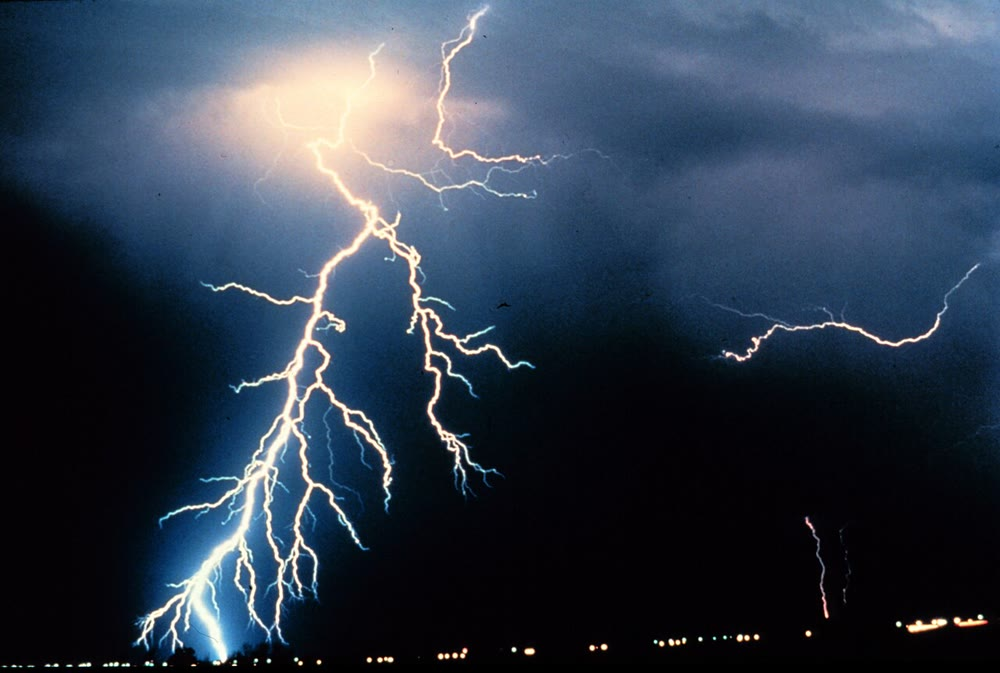
\includegraphics[width=0.62\linewidth]{images/book2/g10-noaa-lightning.jpg}

{\small \omterm{def:g10:storms-and-cyclones:lightning}{Lightning} strokes, between clouds and from the cloud to the ground,
during a night-time \omterm{def:g10:storms-and-cyclones:thunderstorm}{thunderstorm}. Photograph: C.~Clark, NOAA National Severe
Storms Laboratory (public domain).}
\end{omfigure}

Satellites that count the flashes of light over the whole planet find about
1.4 billion \omterm{def:g10:storms-and-cyclones:lightning}{lightning} flashes a year, or 44 every second.
% ledger: christian:flash-rate

\begin{method}[Distance of a storm from flash to thunder]\label{met:g10:storms-and-cyclones:distance}
\begin{enumerate}
  \item The light of the flash arrives practically at once; the thunder
        travels at the speed of sound, about \qty{343}{m/s} at
        \qty{20}{\degreeCelsius}.
  \item Count the seconds $t$ between the flash and the thunder.
  \item The distance is $343\,t$ metres: about \qty{1}{km} for every
        three seconds.
\end{enumerate}
\end{method}
% ledger: const:R, earth:Mmol (speed of sound computed in figdata/grade-10/cyclones.py)

\section{Tornadoes}

\begin{definition}[Tornado]\label{def:g10:storms-and-cyclones:tornado}
A \emph{tornado}\index{tornado} is a violently rotating column of air in
contact with the ground, hanging from the base of a cumulonimbus.
\end{definition}

The strongest \omterm{def:g10:storms-and-cyclones:tornado}{tornadoes} come from \emph{supercells}, \omterm{def:g10:storms-and-cyclones:thunderstorm}{thunderstorms} whose
updraught rotates as a whole. A \omterm{def:g10:storms-and-cyclones:tornado}{tornado} is small and brief: typically a few
hundred metres across, lasting minutes, with an average path of about
\qty{5.6}{km}. But its winds are the strongest at the Earth's surface: a
mobile radar measured about \qty{135}{m/s} (some \qty{480}{km/h}) above the
ground in a \omterm{def:g10:storms-and-cyclones:tornado}{tornado} in Oklahoma in May 1999. The United States has more
\omterm{def:g10:storms-and-cyclones:tornado}{tornadoes} than any other country, around 1200 a year; other regions where
they are frequent include the Canadian prairies, Bangladesh, northern
Argentina and southern Brazil, and Britain.
% ledger: spc:tornado

\begin{omfigure}
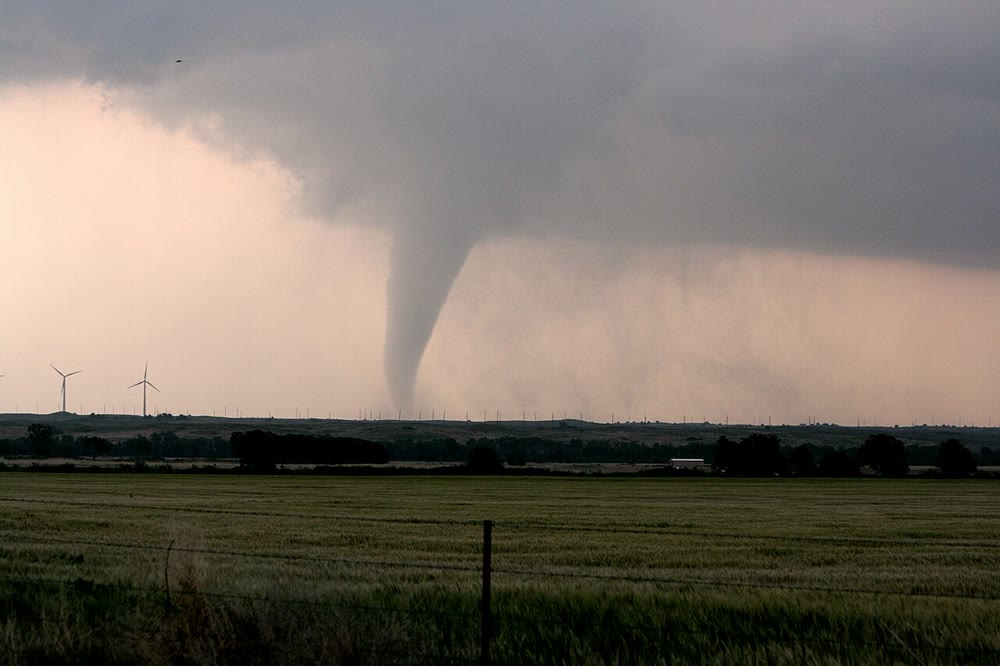
\includegraphics[width=0.62\linewidth]{images/book2/g10-noaa-tornado-kansas.jpg}

{\small A \omterm{def:g10:storms-and-cyclones:tornado}{tornado} over the plains of Kansas, May 2008: the funnel hangs from
the base of the storm cloud. Photograph: Sean Waugh, NOAA National Severe
Storms Laboratory (public domain).}
\end{omfigure}

\section{Tropical cyclones}

\begin{definition}[Tropical cyclone; eye; eyewall]\label{def:g10:storms-and-cyclones:tropical-cyclone}
A \emph{tropical cyclone}\index{tropical cyclone} is a storm, hundreds of
kilometres across, that forms over a warm tropical sea around a centre of
low pressure, with winds spiralling in towards the centre and bands of
\omterm{def:g10:storms-and-cyclones:thunderstorm}{thunderstorms}. When its sustained winds reach \num{64}~knots, about
\qty{119}{km/h}, it is called a hurricane in the Atlantic and the eastern
Pacific, a typhoon in the western Pacific, and simply a cyclone in the Indian
Ocean and the South Pacific. Its calm, nearly cloudless centre is the
\emph{eye}\index{eye}; the ring of towering \omterm{def:g10:storms-and-cyclones:thunderstorm}{thunderstorms} around it, where
the winds are strongest, is the \emph{eyewall}\index{eyewall}.
\end{definition}
% ledger: nhc:sshws

\begin{omfigure}
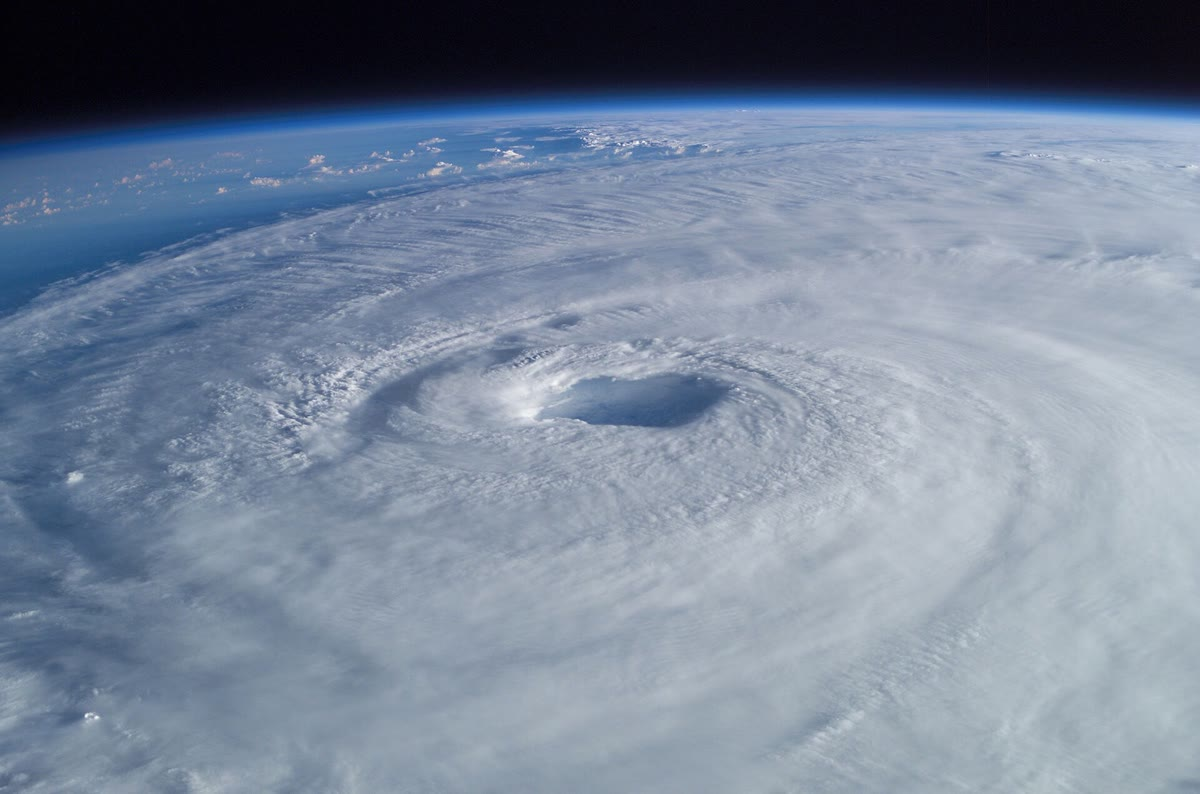
\includegraphics[width=0.78\linewidth]{images/book2/g10-nasa-hurricane-isabel.jpg}

{\small Hurricane Isabel, 15 September 2003, photographed by an astronaut
from the International Space Station: the \omterm{def:g10:storms-and-cyclones:tropical-cyclone}{eye}, the \omterm{def:g10:storms-and-cyclones:tropical-cyclone}{eyewall} and the spiral of
cloud around them. Image: Mike Trenchard, Earth Sciences and Image Analysis
Laboratory, NASA Johnson Space Center (public domain).}
\end{omfigure}

Near the sea surface, humid air flows in towards the low pressure of the
centre. The Earth's rotation deflects moving air to the right in the
Northern Hemisphere: instead of going straight to the centre, the air turns
around it, anticlockwise seen from above (clockwise in the Southern
Hemisphere). Close to the centre it rises in the \omterm{def:g10:storms-and-cyclones:tropical-cyclone}{eyewall}, condenses, and
flows out at the top of the storm. In the \omterm{def:g10:storms-and-cyclones:tropical-cyclone}{eye} a little air sinks, warms and
dries: the sky clears.

\begin{omfigure}
\begin{tikzpicture}[font=\footnotesize, >={Stealth[length=2mm]}]
  \fill[omDef!25] (-6,-0.4) rectangle (6,0);
  \node[anchor=north, omDef!80!black] at (0,-0.05) {warm sea};
  % rain bands
  \foreach \x/\h in {-5.0/1.6, -3.9/2.2, 3.9/2.2, 5.0/1.6}
    \fill[black!10, draw=black!45] (\x-0.35,0.4) -- (\x-0.3,\h) .. controls (\x-0.15,\h+0.35) and (\x+0.15,\h+0.35) .. (\x+0.3,\h) -- (\x+0.35,0.4) -- cycle;
  % eyewall towers and outflow canopy
  \fill[black!14, draw=black!50] (-2.4,0.4) -- (-2.5,4.0) -- (-5.8,4.3) -- (-5.6,4.7) -- (-1.0,4.9) -- (-0.75,4.0) -- (-0.8,0.4) -- cycle;
  \fill[black!14, draw=black!50] (2.4,0.4) -- (2.5,4.0) -- (5.8,4.3) -- (5.6,4.7) -- (1.0,4.9) -- (0.75,4.0) -- (0.8,0.4) -- cycle;
  % inflow, rise, outflow, eye subsidence
  \draw[->, thick, omThm!80!black] (-5.8,0.2) -- (-1.3,0.2) -- (-1.3,4.3) -- (-4.2,4.45);
  \draw[->, thick, omThm!80!black] (5.8,0.2) -- (1.3,0.2) -- (1.3,4.3) -- (4.2,4.45);
  \draw[->, thick, omDef!80!black] (0,4.3) -- (0,1.0);
  \node[anchor=south, align=center] at (0,5.0) {eye: sinking\\dry air};
  \node[anchor=south east, align=right] at (-2.6,4.95) {eyewall};
  \node[anchor=west, align=left] at (-5.95,2.9) {rain\\bands};
  \node[anchor=north, align=center] at (-3.6,0.15) {humid inflow};
  \node[anchor=south east, align=right] at (5.8,4.95) {outflow aloft};
  % plan view
  \begin{scope}[shift={(8.4,2.3)}]
    \draw[black!40] (0,0) circle (1.7);
    \foreach \a in {0,90,180,270}
      \draw[->, thick, omThm!80!black, domain=0:200, samples=30, variable=\t]
        plot ({(1.6-0.0045*\t)*cos(\a+\t)}, {(1.6-0.0045*\t)*sin(\a+\t)});
    \fill[white, draw=black!50] (0,0) circle (0.22);
    \node[anchor=north, align=center] at (0,-1.8) {seen from above\\(Northern Hemisphere)};
  \end{scope}
\end{tikzpicture}

{\small A \omterm{def:g10:storms-and-cyclones:tropical-cyclone}{tropical cyclone} in cross-section (schematic, height greatly
exaggerated): humid air flows in over the warm sea, rises in the \omterm{def:g10:storms-and-cyclones:tropical-cyclone}{eyewall} and
the rain bands, and flows out at the top; a little air sinks in the \omterm{def:g10:storms-and-cyclones:tropical-cyclone}{eye}.
Right: seen from above in the Northern Hemisphere, the inflow turns
anticlockwise around the centre.}
\end{omfigure}

\omterm{def:g10:storms-and-cyclones:tropical-cyclone}{Tropical cyclones} need a warm ocean: water of at least about
\qty{27}{\degreeCelsius} at the surface, warm to a depth of some
\qty{46}{m}. They do not form on the equator itself, where the Earth's
rotation gives the inflowing air no turn: a storm must be at least about
\qty{480}{km} from the equator for the spin to start.
% ledger: aoml:formation

\begin{omfigure}
\begin{tikzpicture}
\begin{axis}[ommap, width=\linewidth, xtick={-180,-120,...,180}, ytick={-60,-30,0,30,60},
  ymin=-70, ymax=70, unbounded coords=jump]
\addplot[fill=omLithAlluv, draw=black!45, line width=0.2pt] table {figdata/out/shared-geo-land.dat};
\addplot[omThm!70, line width=0.25pt] table {figdata/out/grade-10-cyclones-tracks.dat};
\addplot[only marks, mark=*, mark size=0.45pt, omDef!90!black] table {figdata/out/grade-10-cyclones-genesis.dat};
\addplot[black!45, dashed, domain=-180:180] {0};
\end{axis}
\end{tikzpicture}

{\small \omterm{def:g10:storms-and-cyclones:tropical-cyclone}{Tropical cyclones}: the tracks of all the storms of the 2015--2024
seasons (red), and the place where each storm of the 1980--2024 seasons
first reached tropical-storm strength (blue dots). Data: IBTrACS v04r01,
NOAA National Centers for Environmental Information.}
\end{omfigure}
% ledger: data:b2-ibtracs (all statistics computed in figdata/grade-10/cyclones.py)

The map shows the rule at work. Of the 3\,888 storms of 1980--2024, only 24
reached tropical-storm strength within \qty{5}{\degree} of the equator. Most
form between \qty{10}{\degree} and \qty{30}{\degree} of latitude, then
drift west with the trade winds and curve away towards the poles, where the
cold sea weakens them. The South Atlantic, cooler and less favourable, saw
only three in 45 years. About 87 \omterm{def:g10:storms-and-cyclones:tropical-cyclone}{tropical cyclones} form in an average year,
seven in ten of them in the Northern Hemisphere, and a little over half
reach hurricane strength.

\begin{proposition}[The energy source of a tropical cyclone]\label{prop:g10:storms-and-cyclones:energy}
A \omterm{def:g10:storms-and-cyclones:tropical-cyclone}{tropical cyclone} draws its energy from the warm sea: the \omterm{def:g10:earth-energy-budget:latent-heat}{latent heat} taken
up by evaporation at the sea surface is released in the \omterm{def:g10:storms-and-cyclones:tropical-cyclone}{eyewall} and the rain
bands when the vapour condenses. An average hurricane releases in this way
about \qty{6e14}{W}; only a small fraction of it, about \qty{1.5e12}{W},
goes into the kinetic energy of its winds.
\end{proposition}
% ledger: aoml:energy

\begin{proof}[Justification]
An average hurricane rains \qty{1.5}{cm} a day over a circle of radius
\qty{665}{km}, an area of $\pi \times (665\,000)^2 \approx
\qty{1.39e12}{m^2}$: \qty{2.1e10}{m^3}, or \qty{2.1e13}{kg}, of water a day.
Each kilogram that condenses releases about \qty{2.5}{MJ}: $2.1\times10^{13}
\times 2.5\times10^6 \approx \qty{5.2e19}{J}$ a day, that is
$5.2\times10^{19}/86\,400 \approx \qty{6.0e14}{W}$. The power of the winds
is an estimate from measured wind fields, quoted from the same source.
\end{proof}

The storm works like an engine: heat taken in at the warm sea surface, given
off high up in the cold upper air, part of the difference turned into the
motion of the wind. This is why a \omterm{def:g10:storms-and-cyclones:tropical-cyclone}{tropical cyclone} weakens quickly when it
moves over land or over cold water: it loses its supply of evaporating
water.

\section{Intensity, winds and surges}

\begin{definition}[Saffir--Simpson scale]\label{def:g10:storms-and-cyclones:scale}
The \emph{Saffir--Simpson scale}\index{Saffir--Simpson scale} sorts
hurricanes into five categories by their maximum sustained wind; categories
3 to 5 are \emph{major} hurricanes.
\end{definition}

\begin{center}
\small
\begin{tabular}{cccc}
\hline
category & knots & \unit{m/s} & \unit{km/h} \\
\hline
1 & 64--82 & 33--42 & 119--153 \\
2 & 83--95 & 43--49 & 154--177 \\
3 & 96--112 & 49--58 & 178--208 \\
4 & 113--136 & 58--70 & 209--251 \\
5 & 137 or more & 70 or more & 252 or more \\
\hline
\end{tabular}
\end{center}
% ledger: nhc:sshws (m/s converted with 1 knot = 1852/3600 m/s)

The deeper the low pressure at the centre, the stronger the winds that blow
around it: the pressure difference between the centre and the surroundings
is what drives the air inwards.

\begin{omfigure}
\begin{tikzpicture}
\begin{axis}[omrecord, width=0.86\linewidth, height=6.2cm, xmin=15, xmax=100,
  ymin=860, ymax=1015, xlabel={maximum sustained wind (\unit{m/s})},
  ylabel={minimum central pressure (\unit{hPa})},
  tick label style={font=\small}, label style={font=\small}]
\foreach \w in {32.92, 42.70, 49.39, 58.13, 70.48}
  \edef\temp{\noexpand\draw[black!55, densely dashed] (axis cs:\w,860) -- (axis cs:\w,1015);}\temp
\addplot[only marks, mark=*, mark size=0.6pt, omDef!80!black, opacity=0.6] table[x=wind_ms, y=pmin_hpa] {figdata/out/grade-10-cyclones-scatter.dat};
\addplot[omThm!85!black, thick] table[x=wind_ms, y=pmin_hpa] {figdata/out/grade-10-cyclones-fit.dat};
\node[font=\scriptsize, black!60] at (axis cs:37.8,1008) {1};
\node[font=\scriptsize, black!60] at (axis cs:46.0,1008) {2};
\node[font=\scriptsize, black!60] at (axis cs:53.8,1008) {3};
\node[font=\scriptsize, black!60] at (axis cs:64.3,1008) {4};
\node[font=\scriptsize, black!60] at (axis cs:76,1008) {5};
\end{axis}
\end{tikzpicture}

{\small Each dot is one \omterm{def:g10:storms-and-cyclones:tropical-cyclone}{tropical cyclone} of the 2000--2024 seasons: its
strongest sustained wind and its lowest central pressure. The line is the
best straight-line fit: about \qty{1.6}{hPa} lower for every extra metre per
second. Grey dashed lines: the limits of the Saffir--Simpson categories (numbered
at the top). Data: IBTrACS v04r01, NOAA NCEI.}
\end{omfigure}
% ledger: data:b2-ibtracs, nhc:sshws (fit computed in figdata/grade-10/cyclones.py)

The record of the 1980--2024 storms in the archive belongs to Hurricane
Patricia, off the Pacific coast of Mexico in October 2015: sustained winds
of 185 knots, about \qty{95}{m/s}, and a central pressure of \qty{872}{hPa}.
% ledger: data:b2-ibtracs

\begin{definition}[Storm surge]\label{def:g10:storms-and-cyclones:storm-surge}
A \emph{storm surge}\index{storm surge} is the rise of the sea above its
normal level, tide excluded, caused by a storm: the wind piles water against
the coast, and the low pressure lets the sea bulge up beneath the storm.
\end{definition}

\begin{proposition}[The pressure bulge]\label{prop:g10:storms-and-cyclones:bulge}
Under a storm whose central pressure is $\Delta p$ hectopascals below that
of its surroundings, the sea rises by about $\Delta p$ centimetres.
\end{proposition}

\begin{proof}
Far below the surface the pressure must be the same under the storm and
outside it, otherwise the water would flow. The air above the storm weighs
less by $\Delta p$; a column of seawater of height $h$ makes up for it if
$\rho g h = \Delta p$. For $\Delta p = \qty{1}{hPa} = \qty{100}{Pa}$, with
$\rho = \qty{1025}{kg/m^3}$ and $g = \qty{9.81}{m/s^2}$: $h = 100/(1025
\times 9.81) \approx \qty{0.0099}{m}$, about \qty{1}{cm}.
\end{proof}
% ledger: noaa:seawater-1025, nasa:aquarius-density, const:gn

The bulge is the smaller part of most surges: under a central pressure of
\qty{920}{hPa}, \qty{90}{hPa} below its surroundings, it is about
\qty{0.9}{m}. The wind does the rest, pushing water towards the shore,
especially over a wide, shallow sea floor. Arriving with a high tide, a surge
of several metres can flood low coasts far inland.

\begin{omfigure}
\begin{tikzpicture}[font=\footnotesize, >={Stealth[length=2mm]}]
  \def\surf{(0,0) .. controls (1.5,0) and (2.2,0.5) .. (3.0,0.5) .. controls (3.8,0.5) and (4.6,0.4) .. (5.6,0.5) .. controls (7.2,0.65) and (8.8,1.0) .. (10.25,1.3)}
  \fill[omDef!20] (0,-1.6) -- \surf -- (8.8,-1.6) -- cycle;
  \draw[thick, omDef!80!black] \surf;
  \draw[black!50, dashed] (0,0) -- (9.6,0);
  \node[anchor=north west, black!60] at (0.1,-0.05) {normal sea level};
  \fill[omExo!30, draw=black!60] (8.8,-1.6) -- (10.4,1.6) -- (12.4,1.7) -- (12.4,-1.6) -- cycle;
  \foreach \x in {10.9,11.7} \draw[fill=white, draw=black!60] (\x,1.63) rectangle (\x+0.45,2.03) (\x-0.05,2.03) -- (\x+0.225,2.28) -- (\x+0.5,2.03);
  \draw[<->, omThm!80!black] (3.0,0) -- (3.0,0.5);
  \node[anchor=south east, omThm!80!black, align=right] at (2.8,0.6) {bulge under\\the low pressure};
  \draw[<->, omThm!80!black] (9.4,0) -- (9.4,1.12);
  \node[anchor=south, omThm!80!black, align=center] at (8.9,1.75) {wind set-up\\against the coast};
  \foreach \y in {2.9,3.4} \draw[->, thick, black!60] (4.0,\y) -- (6.4,\y);
  \node[anchor=south] at (5.2,3.45) {onshore wind};
  \node[anchor=south, align=center] at (3.0,1.9) {centre of\\the storm};
  \draw[black!40] (3.0,1.9) -- (3.0,0.65);
\end{tikzpicture}

{\small A \omterm{def:g10:storms-and-cyclones:storm-surge}{storm surge} (schematic, heights greatly exaggerated): the sea rises
by about \qty{1}{cm} for every hectopascal of low pressure beneath the
storm, and the onshore wind piles water against the coast.}
\end{omfigure}

\begin{omfigure}
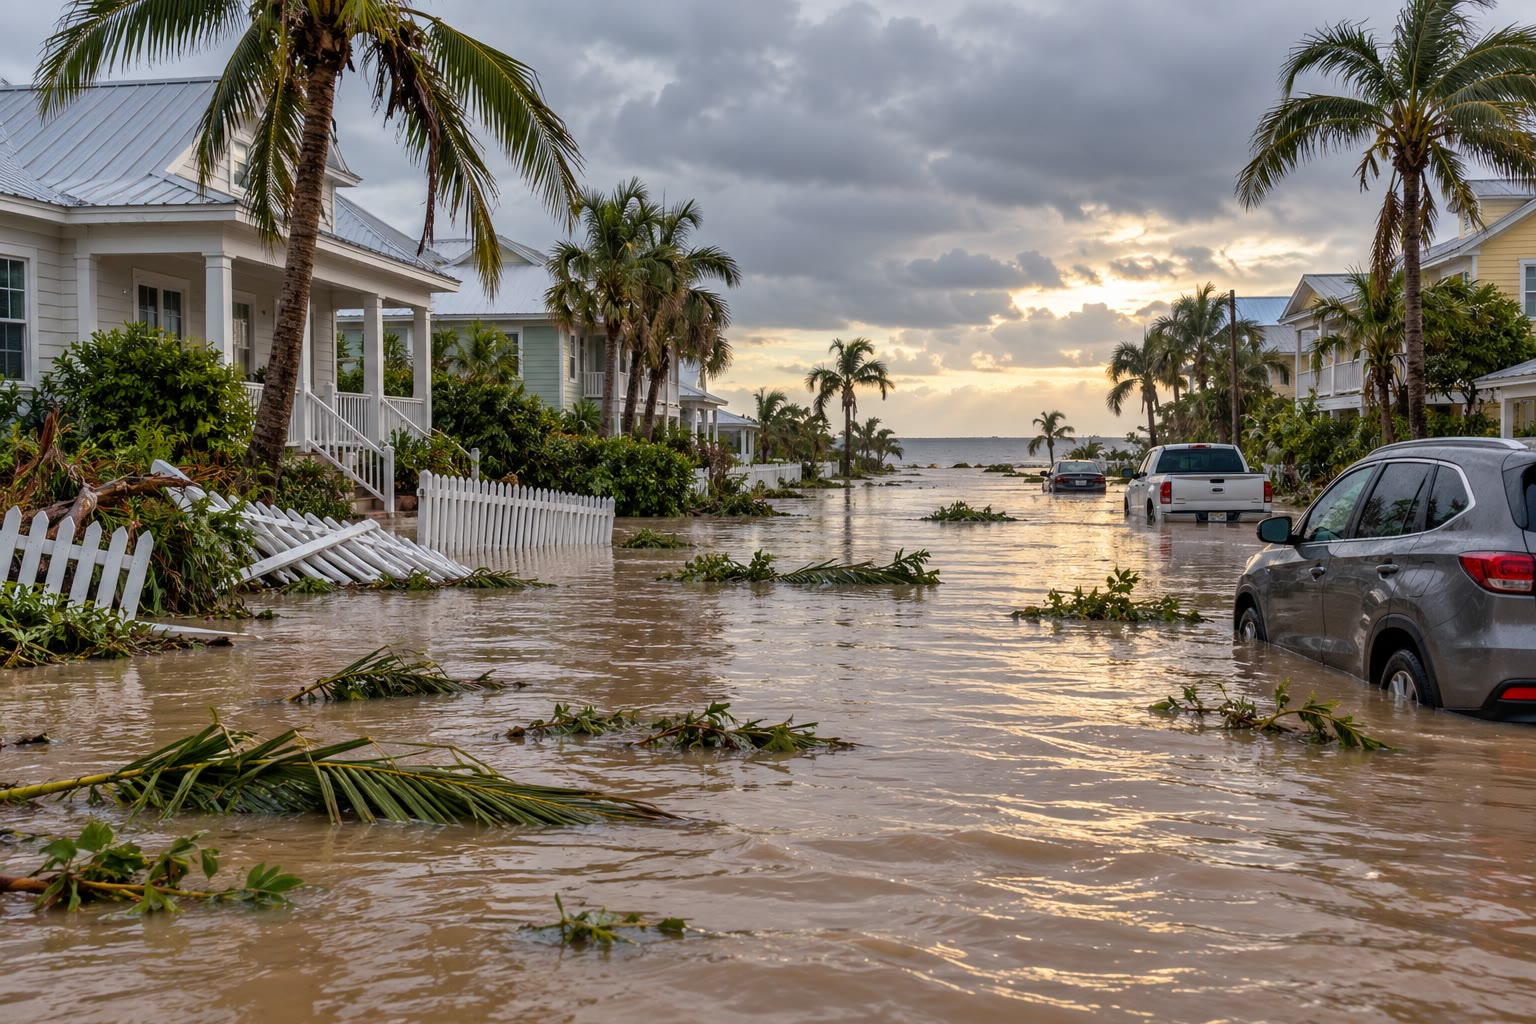
\includegraphics[width=0.7\linewidth]{images/book2/ai/g10-flooded-street.jpg}

{\small A coastal street the morning after a \omterm{def:g10:storms-and-cyclones:storm-surge}{storm surge}: sea water, broken
palms and torn fences.}
\end{omfigure}

\section{Exercises}

\begin{exercise}[$\star$]\label{exo:g10:storms-and-cyclones:1}
Define a \omterm{def:g10:storms-and-cyclones:thunderstorm}{thunderstorm} and \omterm{def:g10:storms-and-cyclones:lightning}{lightning}. What produces the sound of thunder?
\end{exercise}

\begin{exercise}[$\star$]\label{exo:g10:storms-and-cyclones:2}
Define a \omterm{def:g10:storms-and-cyclones:tropical-cyclone}{tropical cyclone}, its \omterm{def:g10:storms-and-cyclones:tropical-cyclone}{eye} and its \omterm{def:g10:storms-and-cyclones:tropical-cyclone}{eyewall}. Where are its winds
strongest?
\end{exercise}

\begin{exercise}[$\star$]\label{exo:g10:storms-and-cyclones:3}
In which Saffir--Simpson category is a hurricane with sustained winds of
\num{70}~knots? Of \num{120}~knots? Of \num{140}~knots? Which of them are
major hurricanes?
\end{exercise}

\begin{exercise}[$\star$]\label{exo:g10:storms-and-cyclones:4}
You count \num{9} seconds between a flash and its thunder, then \num{15}
seconds for the next flash. How far away was each, and is the storm coming
closer?
\end{exercise}

\begin{exercise}[$\star$]\label{exo:g10:storms-and-cyclones:5}
Explain why a tree standing alone in a field is a dangerous shelter in a
\omterm{def:g10:storms-and-cyclones:thunderstorm}{thunderstorm}, and where you should go instead.
\end{exercise}

\begin{exercise}[$\star\star$]\label{exo:g10:storms-and-cyclones:6}
One knot is \qty{1852}{m} per hour. Convert \num{64}~knots and
\num{137}~knots into \unit{m/s} and into \unit{km/h}.
\end{exercise}

\begin{exercise}[$\star\star$]\label{exo:g10:storms-and-cyclones:7}
There are 44 \omterm{def:g10:storms-and-cyclones:lightning}{lightning} flashes a second on the Earth. How many is that in a
day, and in a year?
\end{exercise}

\begin{exercise}[$\star\star$]\label{exo:g10:storms-and-cyclones:8}
A hurricane has a central pressure of \qty{935}{hPa} in surroundings at
\qty{1010}{hPa}. How high is the pressure bulge of the sea beneath it?
\end{exercise}

\begin{exercise}[$\star\star$]\label{exo:g10:storms-and-cyclones:9}
Using the map of tracks, describe where \omterm{def:g10:storms-and-cyclones:tropical-cyclone}{tropical cyclones} form and where
they go after forming. Why are they absent from the equator itself?
\end{exercise}

\begin{exercise}[$\star\star$]\label{exo:g10:storms-and-cyclones:10}
The straight line of the pressure--wind chart is $p \approx 1031 - 1.56\,v$
($p$ in \unit{hPa}, $v$ in \unit{m/s}). What central pressure does it give
for the lower limit of category 5, \qty{70}{m/s}? For a storm of
\qty{40}{m/s}?
\end{exercise}

\begin{exercise}[$\star\star$]\label{exo:g10:storms-and-cyclones:11}
Explain why a \omterm{def:g10:storms-and-cyclones:tropical-cyclone}{tropical cyclone} weakens quickly when it moves over land, and
why it weakens over cold water.
\end{exercise}

\begin{exercise}[$\star\star\star$]\label{exo:g10:storms-and-cyclones:12}
The speed of sound in air is $\sqrt{1.4\,R\,T/M}$, with $R =
\qty{8.314}{J.mol^{-1}.K^{-1}}$, $T$ in kelvin and $M =
\qty{0.02897}{kg/mol}$. Compute it at \qty{0}{\degreeCelsius} and at
\qty{30}{\degreeCelsius}. For a delay of \qty{9}{s}, how much do the two
distances differ? Is the rule ``\qty{3}{s} per kilometre'' good enough?
\end{exercise}

\begin{exercise}[$\star\star\star$]\label{exo:g10:storms-and-cyclones:13}
A \omterm{def:g10:storms-and-cyclones:storm-surge}{storm surge} of \qty{4.0}{m} is measured on a coast as a hurricane with a
central pressure of \qty{940}{hPa} (surroundings \qty{1010}{hPa}) comes
ashore. How much of the surge is due to the pressure bulge, and how much to
the wind? If it arrives at high tide, \qty{1.5}{m} above mean sea level, how
high above mean sea level does the water reach?
\end{exercise}

\begin{exercise}[$\star\star\star$]\label{exo:g10:storms-and-cyclones:14}
A \omterm{def:g10:storms-and-cyclones:tornado}{tornado} turns with winds of \qty{90}{m/s} at \qty{100}{m} from its axis;
a hurricane with winds of \qty{60}{m/s} in an \omterm{def:g10:storms-and-cyclones:tropical-cyclone}{eyewall} \qty{30}{km} from the
centre. How long does the air take to go once round in each case? Compare.
\end{exercise}

\begin{exercise}[$\star\star\star$]\label{exo:g10:storms-and-cyclones:15}
Of the 3\,888 \omterm{def:g10:storms-and-cyclones:tropical-cyclone}{tropical cyclones} of 1980--2024, 24 reached tropical-storm
strength within \qty{5}{\degree} of the equator, 414 within
\qty{10}{\degree}, and 121 beyond \qty{30}{\degree}. Compute the three
percentages. The band within \qty{5}{\degree} of the equator covers about
\qty{9}{\percent} of the Earth's surface: what would you expect if latitude
did not matter, and what do you conclude?
\end{exercise}

\section{Problem: The Heat Engine of a Hurricane}

\begin{problem}[{Weekend problem --- from a day's rain to the power of the
wind}]
\label{pb:g10:storms-and-cyclones:1}
% ledger: aoml:energy, nist:water-latent, earth:Rmean, ipcc:budget-toa (all results computed in figdata/grade-10/cyclones.py or from the rounded data below)
An average hurricane rains \qty{1.5}{cm} a day over a circle of radius
\qty{665}{km}. Use a \omterm{def:g10:earth-energy-budget:latent-heat}{latent heat} of \qty{2.5}{MJ/kg}, a density of water of
\qty{1000}{kg/m^3}, \qty{86400}{s} in a day, and the power of the winds of
an average hurricane, \qty{1.5e12}{W}.

\medskip
\noindent\textbf{Part I --- A day's rain.}
\begin{enumerate}
  \item Compute the area of the circle.
  \item Compute the volume of rain that falls on it in a day.
  \item Express it in cubic kilometres.
  \item Compute its mass.
\end{enumerate}

\medskip
\noindent\textbf{Part II --- The heat released.}
\begin{enumerate}[resume]
  \item Compute the \omterm{def:g10:earth-energy-budget:latent-heat}{latent heat} released in a day by the condensation of
        this water.
  \item Convert it into a power.
  \item The whole Earth absorbs about \qty{1.22e17}{W} of sunlight
        (\cref{ch:g10:earth-energy-budget}). What fraction of it does one
        hurricane release?
  \item The average sunlight absorbed is \qty{240}{W/m^2}. Compute the
        sunlight absorbed by the area of the storm and compare it with the
        storm's \omterm{def:g10:earth-energy-budget:latent-heat}{latent heat}.
  \item What does this comparison show about where the storm's energy was
        gathered?
\end{enumerate}

\medskip
\noindent\textbf{Part III --- Where the water comes from.}
\begin{enumerate}[resume]
  \item What mass of water must evaporate each day to feed this rain?
  \item The average evaporation of the Earth's surface carries
        \qty{82}{W/m^2}. Over what area would average evaporation supply the
        storm's \omterm{def:g10:earth-energy-budget:latent-heat}{latent heat}? Compare with the area of the storm.
  \item Using the table of saturation contents of
        \cref{ch:g10:why-clouds-form}, compare the water that saturated air
        holds at \qty{28}{\degreeCelsius} and at \qty{20}{\degreeCelsius}.
  \item Explain why \omterm{def:g10:storms-and-cyclones:tropical-cyclone}{tropical cyclones} form only over warm seas.
  \item Explain why they weaken over land.
\end{enumerate}

\medskip
\noindent\textbf{Part IV --- The wind.}
\begin{enumerate}[resume]
  \item Compute the kinetic energy given to the winds in a day.
  \item Convert the lower limit of category 3, \num{96}~knots, into
        \unit{m/s} (\num{1}~knot = \qty{1852}{m/h}).
  \item Air near the sea surface has a density of about
        \qty{1.16}{kg/m^3}. Compute the kinetic energy of one cubic metre of
        it moving at that speed.
  \item Compare the \omterm{def:g10:earth-energy-budget:latent-heat}{latent heat} released in a day with the energy of the
        winds in a day.
  \item What becomes of the rest of the heat released?
  \item What fraction of the heat released by condensation becomes wind?
\end{enumerate}
\end{problem}
